\label{chap:amba}

Detta arbete presenterar AMBA, ett verktyg för att visualisera och styra
symbolisk exekvering som är byggt ovanpå \stoe{}. AMBA kör program med symbolisk
indata och visar ett antal grafer över exekveringen. Dessa grafer visar inte
hela programmet från början, utan uppdateras kontinuerligt under programmets
exekvering. Graferna är består av ett antal noder med metadata sammankopplade
med riktade kanter utan metadata. Nodernas metadata visas vid inzoomning samt i
en separat panel för noden som användaren senast klickade på.

\begin{figure}
    \centering
    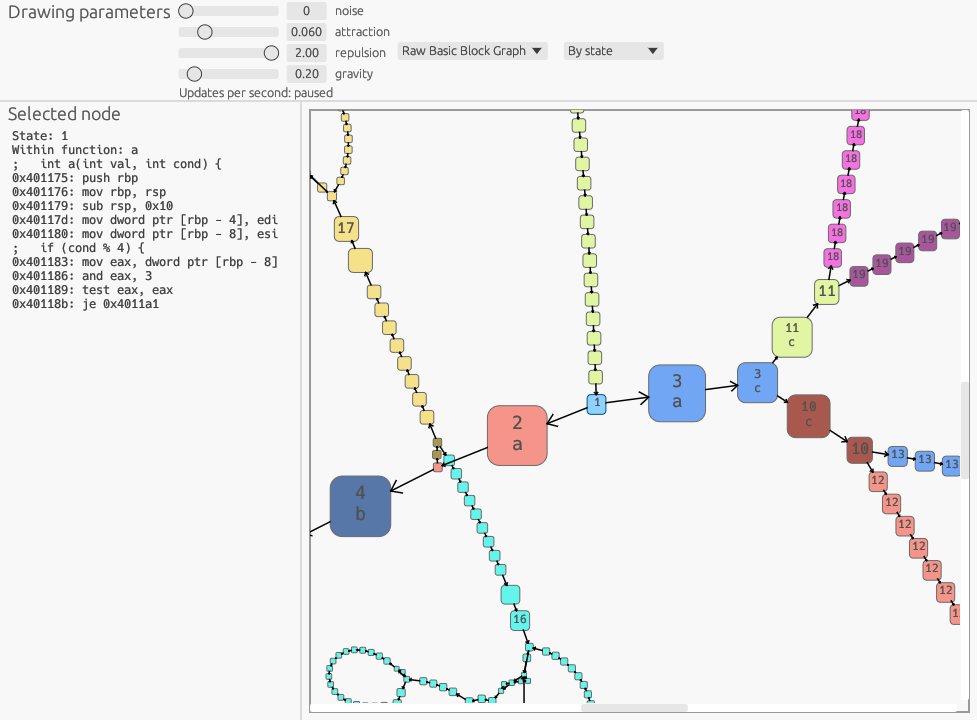
\includegraphics[width=0.7\textwidth]{figures/graph_basic_block.png}\label{fig:graf-basic}
    \caption{AMBAs basic-block-graf för testprogrammet control-flow}
\end{figure}

Den första grafen är en basic-block-graf. Figur~\ref{fig:graf-basic} visar ett
exempel. Här representerar varje tillstånd i grafen ett basic block i
maskinkoden, alltså en sekvens maskinkod som exekveras utan hopp. Det grafiska
gränssnittet visar blockets adress, det symboliska tillståndet blocket exekveras
i och den disassemblerade maskinkoden. Om binären innehåller debugdata visas
även funktionsnamn och om både debugdata och källkoden är tillgänglig visas de
källkodsrader som gett upphov till maskinkoden.

\begin{figure}
    \centering
    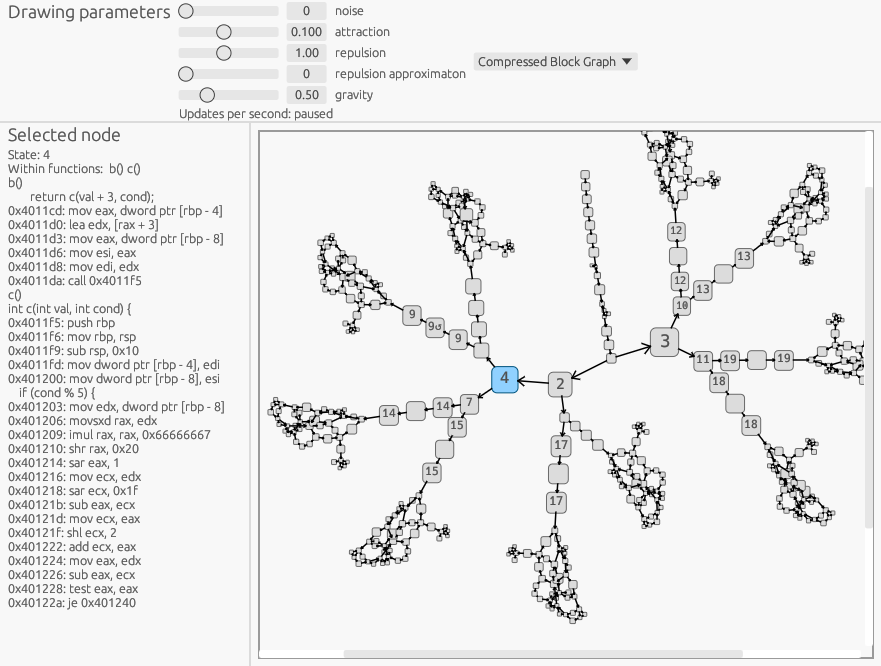
\includegraphics[width=0.7\textwidth]{figures/graph_block_compressed.png}\label{fig:graf-compressed}
    \caption{AMBAs komprimerade basic-block-graf för testprogrammet control-flow}
\end{figure}

Den andra grafen är en komprimerad basic-block-graf.
Figur~\ref{fig:graf-compressed} visar ett exempel. Den visar samma graf som den
första, men med linjesubgrafer sammanslagna till samma nod. Precist uttryckt har
alla kanter anslutna till noder med ingrad och utgrad exakt ett
kantkomprimerats. Sidopanelen visar samma information som för basic-block-grafen, alltså assemblerkod och debugdata, men för hela spannet av sammanslagna noder.

\begin{figure}
    \centering
    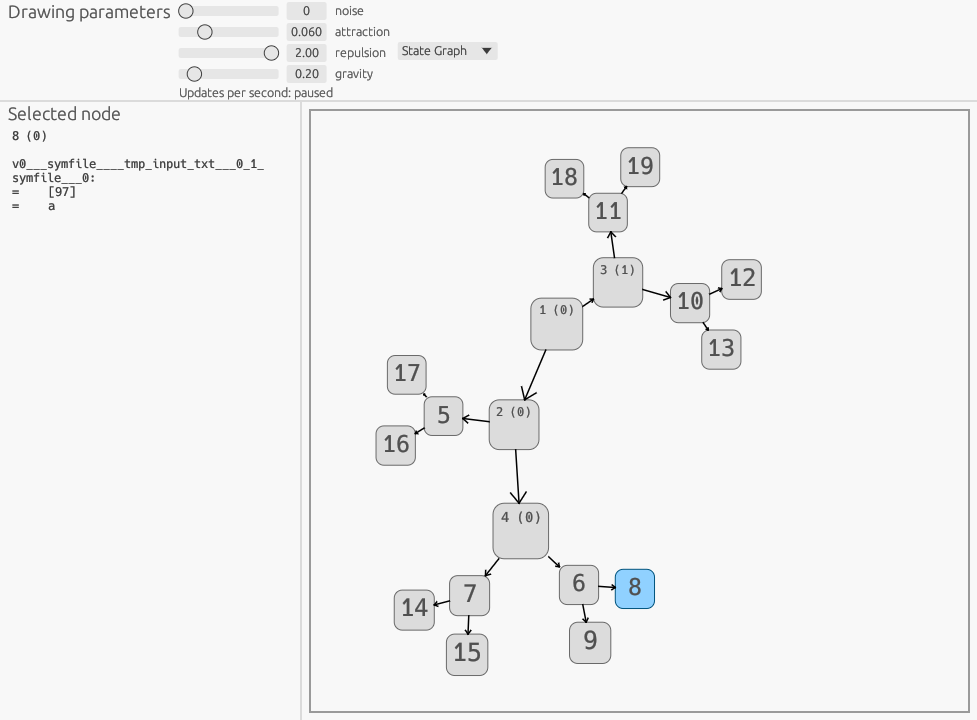
\includegraphics[width=0.7\textwidth]{figures/graph_symbolic.png}\label{fig:graf-symbolic}
    \caption{AMBAs graf över symboliska tillstånd för testprogrammet control-flow}
\end{figure}

Den tredje grafen visar symboliska tillstånd. Figur~\ref{fig:graf-symbolic}
visar ett exempel. Ett tillstånd utgörs av exekveringsspannet uppdelat vid varje
branch som görs baserat på ett symboliskt uttryck. Sidopanelen visar
tillståndets namn samt det grennummer som identiferar det föränderliga
tillståndet i \stoe{}. Då föräldrar inte kan samexitera i tid med sina barn
använder \stoe{} grennummer för att hänvisa till nu körande tillstånd.

Utöver att visa dessa grafer går det också att välja noder i den symboliska
tillståndsgrafen för att prioritera deras fortsatta evaulering. Detta gör det
möjligt att undersöka intressanta subträd i grafer som är större än vad AMBA
realistiskt sett kan besöka och visa. Enorma grafer kan till exempel skapas av
program som inte terminerar.

Grafnodernas placering i 2D hittas genom iterativ lösning för lägst energi i ett
system av attraktion, repulsion och externa krafter. Utplaceringsalgoritmens
parametrar kan konfigureras i realtid vid körning av användaren i toppanelen.
Denna panelen låter även användaren välja vilken graf de vill visa.

Genom \stoe{} kör AMBA det analyserade programmet virtualiserat med KVM i
QEMU.\@ Detta innebär att den analyserade binärens beteende i hög grad inte
påverkas av miljön på datorn som kör AMBA, vilket gör analysern mer
reproducibel. Det innebär också att skadlig kod borde kunna analyseras dynamisk
i AMBA med låg risk för skadlig påverkan på användarens dator. Dock är AMBA
omogen programvara som ej granskats för felkonfiguration eller liknande kopplat
till QEMU eller \stoe{}, så vi rekommenderar inte att använda AMBA för analys av
skadlig kod i dess nuvarande skick.

\subsection{Begränsningar}

Alla program kan inte hanteras av AMBA.\@ Programmen som AMBA kör måste vara
byggda för Linux x86\_64 och kunna köras på Ubuntu-22.04-x86\_64. Detta görs
lättast med att antingen bygga direkt för Ubuntu, eller för bredare support,
fullt statiskt länkad mot t.ex.\ musl.

Den symboliska indatan är också begränsad till att komma ifrån
stdin. Alltså kan inte programargument (argc, argv) eller filer på
disk användas.

\subsection{Hur du kör AMBA}
